\begin{frame}
 \frametitle{L'implémentation}

\begin{itemize}
 \item Langage Java
 \item Utilise des fichiers .data en entrée
 \item Utilisation de la librairie Weka pour l'implémentation de C4.5
\end{itemize}
Usage : \\
java -jar classification.jar --algorithm <algorithm> --source <sourceFile> --percentage <percentage> --classIndex <classIndex> --intervalNumber <intervalNumber>
  \begin{itemize}
    \item algorithm : C45 | NaiveBayes : the algorithm to use 
    \item sourceFile : the input data
    \item percentage : the percentage of data to consider as the training set
    \item classIndex : the index of the class
	\item intervalNumber : the number of intervals k
  \end{itemize}
\end{frame}

 \begin{frame}%[plain]
%\begin{agrandirmarges}{1cm}{1cm}
 \begin{center}

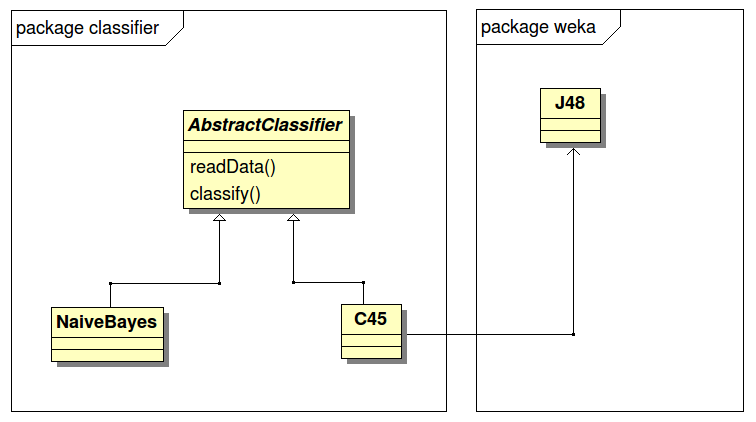
\includegraphics[width=350px]{classDiagram.png}
\end{center}

%\end{agrandirmarges}


\end{frame}
 